\documentclass{article}
\usepackage{graphicx,pdfpages}

\title{CS522: Design Review}
\author{Erin Marshall \texttt{<limarshall@wisc.edu>}}

\begin{document}
\maketitle

\section{Diagrams}
% \includegraphics{overview.pdf}
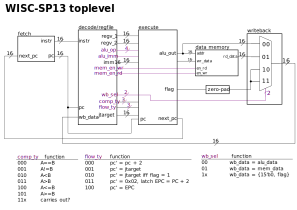
\includepdf[pages=-,fitpaper]{overview.pdf}

\includepdf[pages=-,fitpaper]{fetch.pdf}
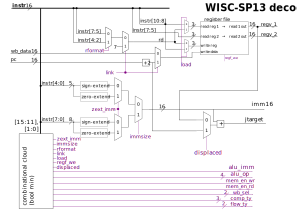
\includepdf[pages=-,fitpaper]{decode.pdf}
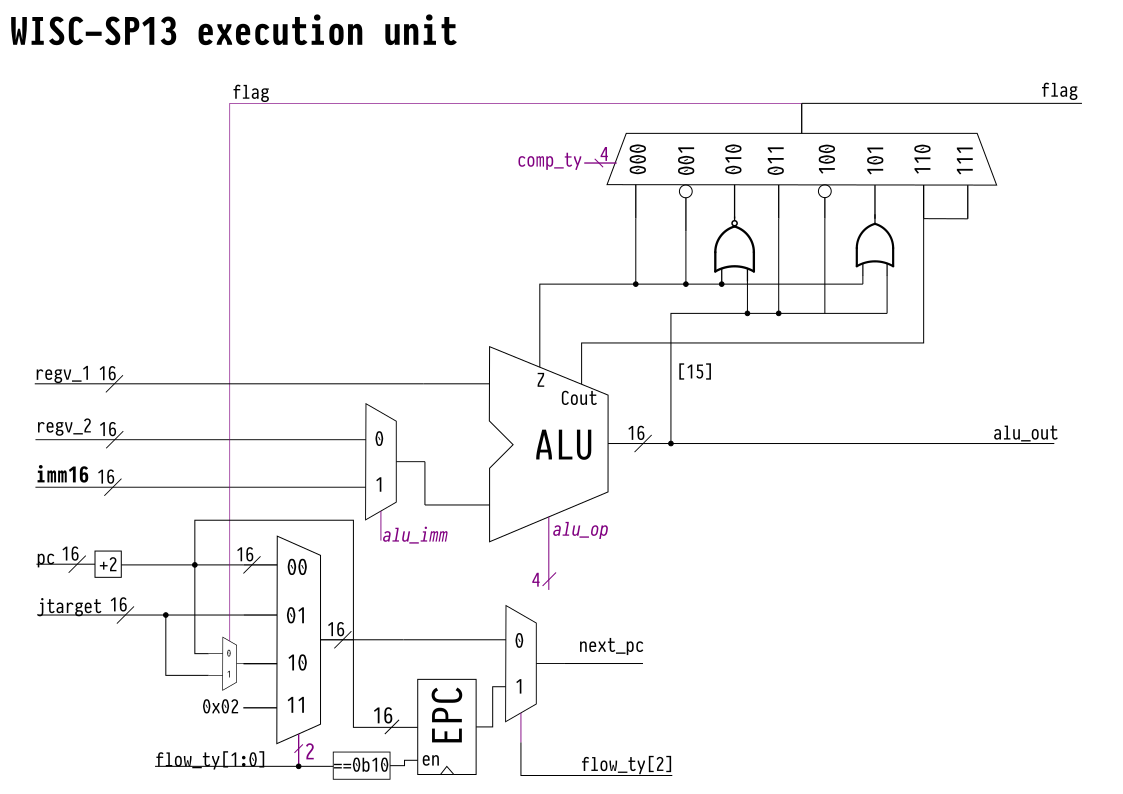
\includepdf[pages=-,fitpaper]{execute.pdf}
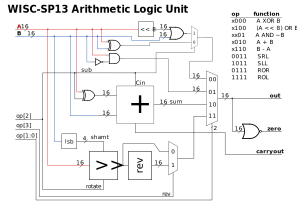
\includepdf[pages=-,fitpaper]{alu.pdf}

\def\headline#1{\hbox to \hsize{\hrulefill\quad\lower.3em\hbox{#1}\quad\hrulefill}}

\section{Control Signals Listing}
\begin{tabular}{lp{1\textwidth}}
	\textbf{signal} & \textbf{description} \\
	alu\_imm & muxes the ALU to ingest \textbf{imm16} as its B input\\
	alu\_op[3:0] & selects an ALU operation to perform. values listed on ALU sheet\\
	mem\_en\_wr & enables a memory write\\
	mem\_en\_rd & enables a memory read\\
	wb\_sel[2:0] & selects which data will be written back to the register file (if it's enabled for writing) \\
	comp\_ty[3:0] & "comparison type"; selects a operation to perform on the output of the ALU to facilitate comparisons (for both set-by-comparison and branches). values listed on toplevel sheet. \\
	flow\_ty & selects control flow type: how the next\_pc is computed in the execute block. values listed on toplevel sheet. \\
	\multicolumn{2}{c}{\headline{\textbf{decode}-block internal control signals}}\\
	rformat & asserted if R-format instruction is being processed; muxes decoding of Rd \\
	link & asserted when a linking jump is being performed; forces Rd = 7 and register writeback data = PC + 2 \\
	load & asserted when load instructions are being performed; swaps Rd field to read port 1 on the register file and Rs to the write reg port. \\
	regf\_we & enables register file writeback \\
	zext\_imm & selects zero-extension for the immediate field \\
	immsize[1:0] & selects between 5, 8, and 11 bit (displacement) immediate fields \\
	displaced & if asserted, jtarget = pc + 2 + imm16; otherwise, jtarget = regv\_1 + imm16. \\
	zero & pushes a zero out of the reg 2 value port, used for ALU ops where B = 0. \\
\end{tabular}

\end{document}